\documentclass[journal,12pt,twocolumn]{IEEEtran}
\usepackage{setspace}
\usepackage{gensymb}
\usepackage{caption}
\singlespacing
\usepackage{csvsimple}
\usepackage{amsmath}
\usepackage{multicol}
\usepackage{amssymb}
\usepackage{newfloat}
\usepackage{listings}
%\usepackage{iithtlc}
\usepackage{color}
\usepackage[colorlinks= true,
			linkcolor = blue,
			urlcolor = blue,
			citecolor = blue
			anchorcolor = blue]{hyperref}
\usepackage{tikz}
\usetikzlibrary{shapes,arrows}
\usepackage{hyperref}
\usepackage{amsthm}
\usepackage{mathrsfs}
\usepackage{txfonts}
\usepackage{stfloats}
\usepackage{cite}
\usepackage{cases}
\usepackage{mathtools}
\usepackage{caption}
\usepackage{enumerate}	
\usepackage{enumitem}
\usepackage{amsmath}

\usepackage{longtable}
\usepackage{multirow}

\usepackage{enumitem}
\usepackage{mathtools}
\usepackage{hyperref}
%\usepackage[framemethod=tikz]{mdframed}
\usepackage{listings}
    %\usepackage[latin1]{inputenc}                                 %%
    \usepackage{color}                                            %%
    \usepackage{array}                                            %%
    \usepackage{longtable}                                        %%
    \usepackage{calc}                                             %%
    \usepackage{multirow}                                         %%
    \usepackage{hhline}                                           %%
    \usepackage{ifthen}                                           %%
  %optionally (for landscape tables embedded in another document): %%
    \usepackage{lscape}     


\usepackage{url}
\def\UrlBreaks{\do\/\do-}


%\usepackage{stmaryrd}


%\usepackage{wasysym}
%\newcounter{MYtempeqncnt}
\DeclareMathOperator*{\Res}{Res}
%\renewcommand{\baselinestretch}{2}
\renewcommand\thesection{\arabic{section}}
\renewcommand\thesubsection{\thesection.\arabic{subsection}}
\renewcommand\thesubsubsection{\thesubsection.\arabic{subsubsection}}

\renewcommand\thesectiondis{\arabic{section}}
\renewcommand\thesubsectiondis{\thesectiondis.\arabic{subsection}}
\renewcommand\thesubsubsectiondis{\thesubsectiondis.\arabic{subsubsection}}

% correct bad hyphenation here
\hyphenation{op-tical net-works semi-conduc-tor}

%\lstset{
%language=C,
%frame=single, 
%breaklines=true
%}

%\lstset{
	%%basicstyle=\small\ttfamily\bfseries,
	%%numberstyle=\small\ttfamily,
	%language=Octave,
	%backgroundcolor=\color{white},
	%%frame=single,
	%%keywordstyle=\bfseries,
	%%breaklines=true,
	%%showstringspaces=false,
	%%xleftmargin=-10mm,
	%%aboveskip=-1mm,
	%%belowskip=0mm
%}

%\surroundwithmdframed[width=\columnwidth]{lstlisting}
\def\inputGnumericTable{}                                 %%
\lstset{
%language=C,
frame=single, 
breaklines=true,
columns=fullflexible
}
 

\begin{document}
%
\tikzstyle{block} = [rectangle, draw,
    text width=3em, text centered, minimum height=3em]
\tikzstyle{sum} = [draw, circle, node distance=3cm]
\tikzstyle{input} = [coordinate]
\tikzstyle{output} = [coordinate]
\tikzstyle{pinstyle} = [pin edge={to-,thin,black}]

\theoremstyle{definition}
\newtheorem{theorem}{Theorem}[section]
\newtheorem{problem}{Problem}
\newtheorem{proposition}{Proposition}[section]
\newtheorem{lemma}{Lemma}[section]
\newtheorem{corollary}[theorem]{Corollary}
\newtheorem{example}{Example}[section]
\newtheorem{definition}{Definition}[section]
%\newtheorem{algorithm}{Algorithm}[section]
%\newtheorem{cor}{Corollary}
\newcommand{\BEQA}{\begin{eqnarray}}
\newcommand{\EEQA}{\end{eqnarray}}
\newcommand{\define}{\stackrel{\triangle}{=}}
\bibliographystyle{IEEEtran}
%\bibliographystyle{ieeetr}
\providecommand{\nCr}[2]{\,^{#1}C_{#2}} % nCr
\providecommand{\nPr}[2]{\,^{#1}P_{#2}} % nPr
\providecommand{\mbf}{\mathbf}
\providecommand{\pr}[1]{\ensuremath{\Pr\left(#1\right)}}
\providecommand{\qfunc}[1]{\ensuremath{Q\left(#1\right)}}
\providecommand{\sbrak}[1]{\ensuremath{{}\left[#1\right]}}
\providecommand{\lsbrak}[1]{\ensuremath{{}\left[#1\right.}}
\providecommand{\rsbrak}[1]{\ensuremath{{}\left.#1\right]}}
\providecommand{\brak}[1]{\ensuremath{\left(#1\right)}}
\providecommand{\lbrak}[1]{\ensuremath{\left(#1\right.}}
\providecommand{\rbrak}[1]{\ensuremath{\left.#1\right)}}
\providecommand{\cbrak}[1]{\ensuremath{\left\{#1\right\}}}
\providecommand{\lcbrak}[1]{\ensuremath{\left\{#1\right.}}
\providecommand{\rcbrak}[1]{\ensuremath{\left.#1\right\}}}
\theoremstyle{remark}
\newtheorem{rem}{Remark}
\newcommand{\sgn}{\mathop{\mathrm{sgn}}}
\providecommand{\abs}[1]{\left\vert#1\right\vert}
\providecommand{\res}[1]{\Res\displaylimits_{#1}} 
\providecommand{\norm}[1]{\left\Vert#1\right\Vert}
\providecommand{\mtx}[1]{\mathbf{#1}}
\providecommand{\mean}[1]{E\left[ #1 \right]}
\providecommand{\fourier}{\overset{\mathcal{F}}{ \rightleftharpoons}}
%\providecommand{\hilbert}{\overset{\mathcal{H}}{ \rightleftharpoons}}
\providecommand{\system}{\overset{\mathcal{H}}{ \longleftrightarrow}}
	%\newcommand{\solution}[2]{\textbf{Solution:}{#1}}
\newcommand{\solution}{\noindent \textbf{Solution: }}
\newcommand{\myvec}[1]{\ensuremath{\begin{pmatrix}#1\end{pmatrix}}}
\providecommand{\dec}[2]{\ensuremath{\overset{#1}{\underset{#2}{\gtrless}}}}
\DeclarePairedDelimiter{\ceil}{\lceil}{\rceil}
%\numberwithin{equation}{section}
%\numberwithin{problem}{subsection}
%\numberwithin{definition}{subsection}
\makeatletter
\@addtoreset{figure}{section}
\makeatother
\let\StandardTheFigure\thefigure
\renewcommand{\thefigure}{\thesection}
\numberwithin{problem}{section}
\makeatletter
\@addtoreset{table}{section}
\makeatother
\let\StandardTheFigure\thefigure
\let\StandardTheTable\thetable
\let\vec\mathbf
\numberwithin{equation}{section}
\vspace{3cm}
\title{
	\logo{
	Random Numbers
	}
}

\author{Aniket Tukaram Satpute}

%\maketitle
\begin{abstract}
This manual provides a simple introduction to the generation of random numbers
\end{abstract}
%%
\section{Uniform Random Numbers}
Let $U$ be a uniform random variable between 0 and 1.
\begin{enumerate}[label=\thesection.\arabic*
,ref=\thesection.\theenumi]
%1.1
\item Generate $10^6$ samples of $U$ using a C program and save into a file called uni.dat .
\\
\solution : Link to the code : \href{https://github.com/anikettsatpute/Probability-and-Random-Variable-Assignment/blob/main/code/code1_1.c}{C code}
%
\vspace{0.2in}
%1.2
\item
Load the uni.dat file into python and plot the empirical CDF of $U$ using the samples in uni.dat. The CDF is defined as
\begin{align}
F_{U}(x) = \pr{U \le x}
\end{align}
\\
\solution  The following code plots Fig: \href{https://github.com/anikettsatpute/Probability-and-Random-Variable-Assignment/blob/main/code/code1_2.py}{Python code} 
\begin{figure}[h]
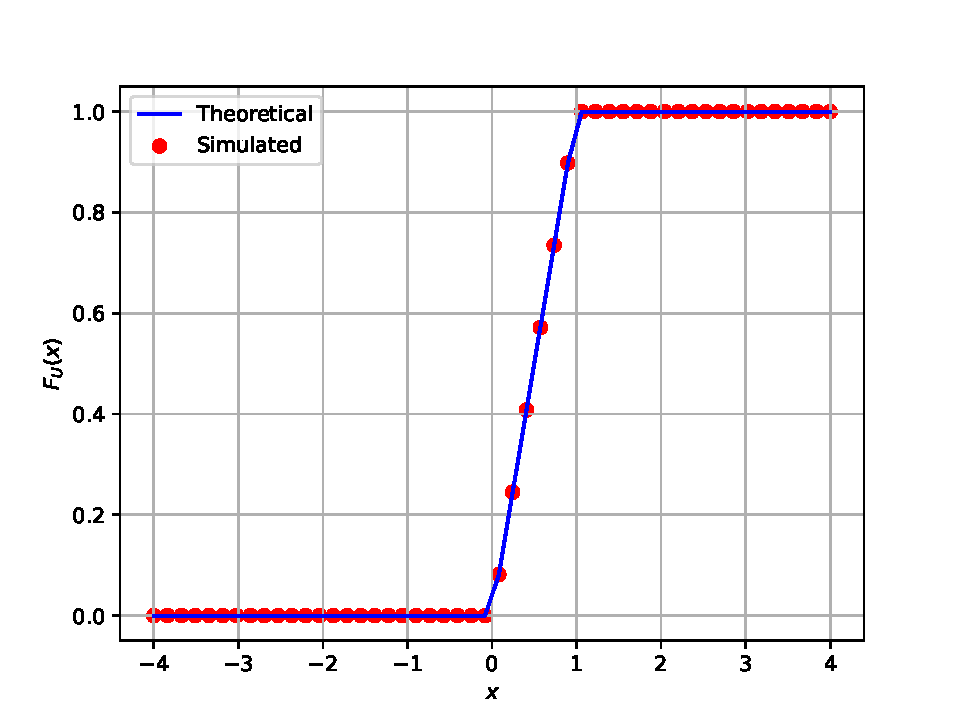
\includegraphics[width=\columnwidth]{../Figures/uni_cdf}
\caption{The CDF of $U$}
\label{fig:uni_cdf}
\end{figure}
%
%1.3
\item
Find a  theoretical expression for $F_{U}(x)$.\\
\solution As U is uniformly distributed random variable in the interval (0,1) and
\begin{align}
p_U(x) = 
\begin{cases}
1, & x \in (0, 1) \\
0, & otherwise
\end{cases}
\end{align}
\begin{align}
F_U(x) &= \int_{-\infty}^{x} p_U(x)dx
\end{align}
\begin{align}
F_U(x) = 
\begin{cases}
0, & x \in (-\infty,0) \\
x, & x \in (0,1)\\
1, & x \in (1,\infty)
\end{cases}
\end{align}

%1.4
\item
The mean of $U$ is defined as
\begin{equation}
E\sbrak{U} = \frac{1}{N}\sum_{i=1}^{N}U_i
\end{equation}
and its variance as
\begin{equation}
\text{var}\sbrak{U} = E\sbrak{U- E\sbrak{U}}^2 
\end{equation}
Write a C program to  find the mean and variance of $U$.\\

\solution Link to the code :\href{https://github.com/anikettsatpute/Probability-and-Random-Variable-Assignment/blob/main/code/code1_4.c}{C code}

\begin{figure}[h]
\centering
\includegraphics[width=\columnwidth]{../fig/screen15.png}
\caption{Output}
\label{fig:gauss_cdf}
\end{figure}

%1.5
\item Verify your result theoretically given that
\end{enumerate}

\begin{equation}
E\sbrak{U^k} = \int_{-\infty}^{\infty}x^kdF_{U}(x)
\end{equation}

\solution we know that,
\begin{equation}
dF_{U}(x) = p_U(x)dx
\end{equation}
also mean ($\mu$) is E(U):
Hence,
\begin{align*}
\mu &= \int_{-\infty}^{\infty}xp_{U}(x)dx\\
&= \int_{0}^{1}xdx\\
&= \frac{x^2}{2} \Bigg|^{1}_{0} \\
&= \frac{1}{2}
\end{align*}
Variance($\sigma^{2}$) = $E(U^{2}) - E(U)^{2}$
\begin{align*}
E(U^{2}) &= \int_{-\infty}^{\infty}x^{2}p_{U}(x)dx\\
&= \int_{0}^{1}x^{2}dx\\
&= \frac{x^3}{3} \Bigg|^{1}_{0} \\
&= \frac{1}{3}
\end{align*}
\begin{align*}
\sigma^{2} &= \frac{1}{3} - \frac{1}{4}\\
&= \frac{1}{12}
\end{align*}
\vspace{0.3in}
\section{Central Limit Theorem}
%
\begin{enumerate}[label=\thesection.\arabic*
,ref=\thesection.\theenumi]



%2.1
\item
Generate $10^6$ samples of the random variable
\begin{equation}
X = \sum_{i=1}^{12}U_i -6
\end{equation}
using a C program, where $U_i, i = 1,2,\dots, 12$ are  a set of independent uniform random variables between 0 and 1
and save in a file called gau.dat\\
\solution  link to the code :\href{https://github.com/anikettsatpute/Probability-and-Random-Variable-Assignment/blob/main/code/code2_1.c}{C code}
\vspace{0.2in}

%2.2
\item
Load gau.dat in python and plot the empirical CDF of $X$ using the samples in gau.dat. What properties does a CDF have?
\\
\solution Link to Python code :\href{https://github.com/anikettsatpute/Probability-and-Random-Variable-Assignment/blob/main/code/code2_2.py}{Python code}

\begin{figure}[h]
\centering
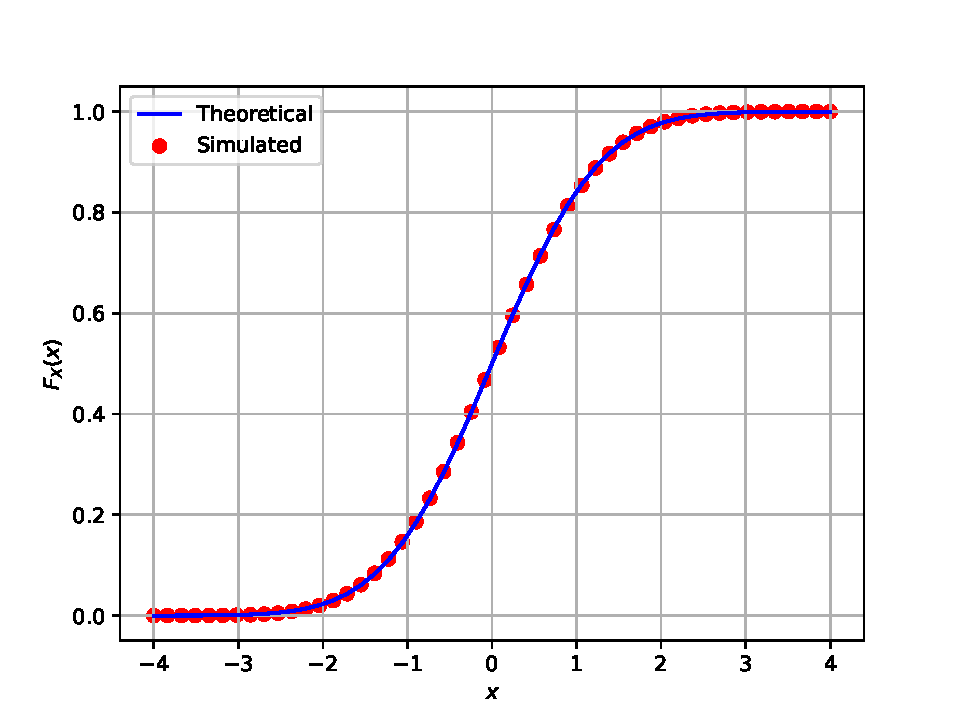
\includegraphics[width=\columnwidth]{../Figures/gau_cdf}
\caption{The CDF of $X$}
\label{fig:gau_cdf}
\end{figure}

Properties:\\
(1)  Graph is symmetric about a single point\\
(2)	 The $F_X(x)$ is non-decreasing function\\
(3)	 $\lim_{x \to \infty} F_X(x)$
\vspace{0.2in}

%2.3
\item
Load gau.dat in python and plot the empirical PDF of $X$ using the samples in gau.dat. The PDF of $X$ is defined as
\begin{align}
p_{X}(x) = \frac{d}{dx}F_{X}(x)
\end{align}
What properties does the PDF have?
\\
\solution Link to the code :\href{https://github.com/anikettsatpute/Probability-and-Random-Variable-Assignment/blob/main/code/code2_3.py}{Python code}

\begin{figure}[h]
\centering
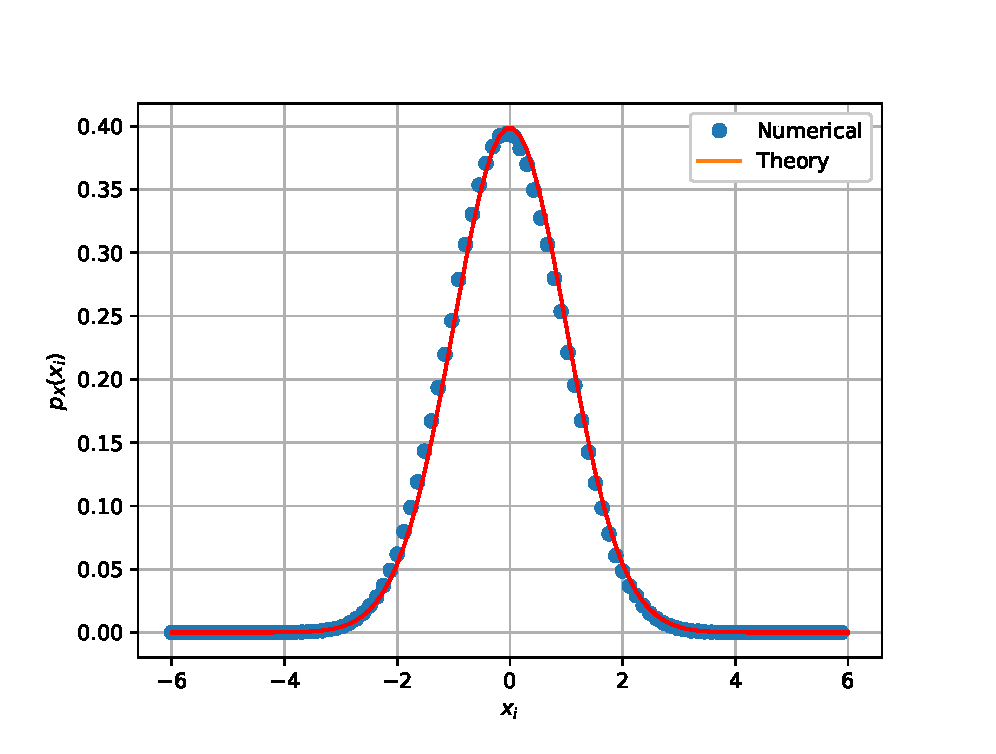
\includegraphics[width=\columnwidth]{../Figures/gauss_pdf}
\caption{The PDF of $X$}
\label{fig:gauss_pdf}
\end{figure}

Properties :\\
(1) Area under the curve is One.\\
(2) Symmetric about line $x=\mu$.\\
(3) Increasing in first half and decreasing in other half.

\vspace{0.2in}

%2.4
\item Find the mean and variance of $X$ by writing a C program.\\
\solution Link to the code :\href{https://github.com/anikettsatpute/Probability-and-Random-Variable-Assignment/blob/main/code/code2_4.c}{C code}
\begin{figure}[h]
\centering
\includegraphics[width=\columnwidth]{../fig/screen25.png}
\caption{Output}
\label{fig:gauss_cdf}
\end{figure}

%2.5
\item Given that
\begin{align}
p_{X}(x) = \frac{1}{\sqrt{2\pi}}\exp\brak{-\frac{x^2}{2}}, -\infty < x < \infty,
\end{align}
repeat the above exercise theoretically.
\solution \\
(1) CDF is 
\begin{align*}
F_X(x) &= \int_{-\infty}^{x}p_X(x)dx\\
&= 1
\end{align*}
(2) Mean is
\begin{align*}
\mu = E(x) = \int_{-\infty}^{\infty} x p_X(x)dx\\
\end{align*}
Due to symmetry clearly, $\mu = 0$\\

(3) Variance is
\begin{align*}
var[X] &= E(X^{2}) - E(X)^{2}\\
&= \int_{-\infty}^{\infty} x^{2} p_X(x)dx  - 0\\
&= 1
\end{align*}
(4) Q function is 
\begin{align*}
Q(x) &= Pr(x>X)\\
&= 1 - F_X(x)
\end{align*}
Then CDF is:
\begin{align*}
F_X(x) &= 1 - Q(x)\\
\end{align*}
\end{enumerate}
\section{From Uniform to Other}
\begin{enumerate}[label=\thesection.\arabic*
,ref=\thesection.\theenumi]

%3.1
\item
Generate samples of 

\begin{equation}
V = -2\ln\brak{1-U}
\end{equation}

and plot its CDF. \\
\solution Link to the code :\href{https://github.com/anikettsatpute/Probability-and-Random-Variable-Assignment/blob/main/code/code3_2.c}{Python code}
\begin{figure}[h]
\centering
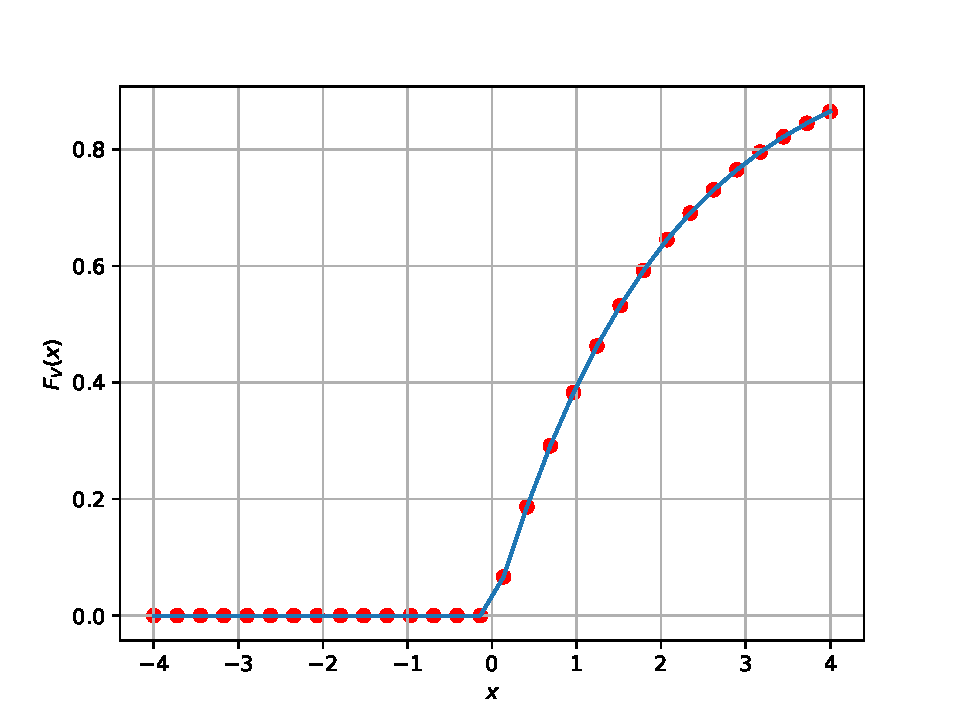
\includegraphics[width=\columnwidth]{../Figures/3_1_cdf}
\caption{CDF of V}
\label{fig:gauss_pdf}
\end{figure}

%3.2
\item Find a theoretical expression for $F_V(x)$.\\
\solution \\
\begin{align*}
F_V(X) &= Pr(V \le x)\\
&= Pr(-2 \ln(1-U) \le x)\\
&= Pr((1-U) \ge \exp(\frac{-x}{2})\\
&= Pr(U \le (1-\exp(\frac{-x}{2}))\\
&= F_U(1-\exp \frac{-x}{2})
\end{align*} 
from equation (1.3),
\begin{align*}
F_U(x) = 
\begin{cases}
0, & x \in (-\infty,0) \\
(1-\exp \frac{-x}{2}), & x \in (0,\infty)
\end{cases}
\end{align*}
\end{enumerate}
\section{Triangular Distribution}
\begin{enumerate}[label=\thesection.\arabic*
,ref=\thesection.\theenumi]

%4.1
\item Generate
\begin{equation}
T = U_1 + U_2
\end{equation}
\solution Link to the code :\href{https://github.com/anikettsatpute/Probability-and-Random-Variable-Assignment/blob/main/code/code4_1.c}{C code}
\vspace{0.2in}

%4.2
\item Find CDF of T\\
\solution Link to the code :\href{https://github.com/anikettsatpute/Probability-and-Random-Variable-Assignment/blob/main/code/code4_2.py}{Pyhton code}\\

\begin{figure}[h]
\centering
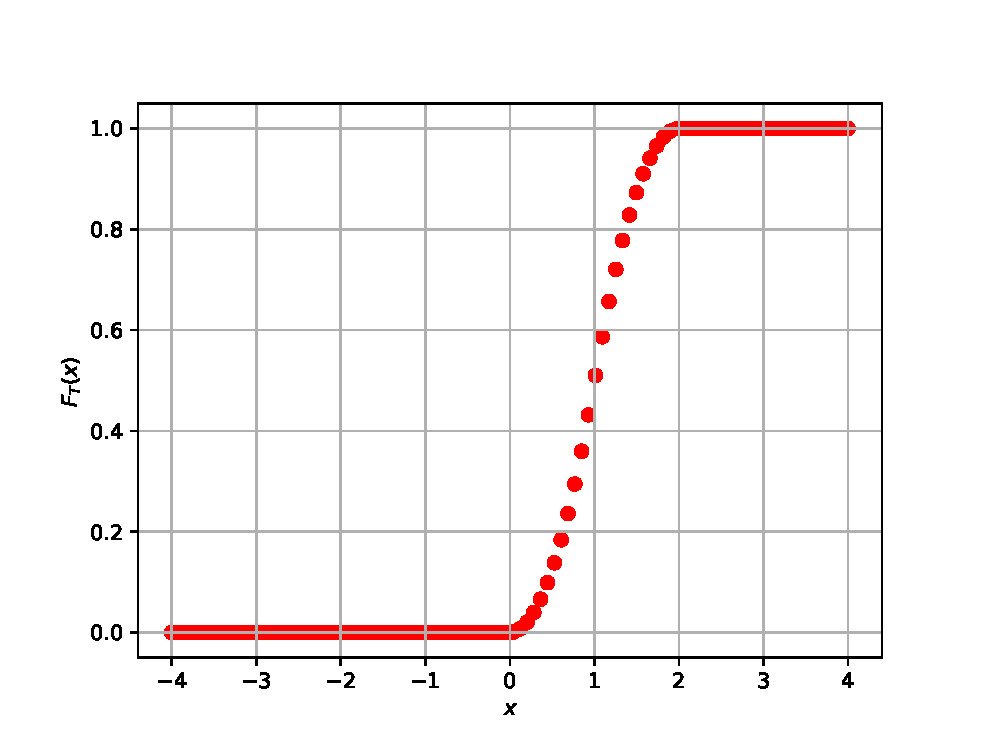
\includegraphics[width=\columnwidth]{../Figures/4_2_CDF}
\caption{CDF of T}
\label{fig:gauss_pdf}
\end{figure}

%4.3
\item Find the PDF of T.\\
\solution Link to the code :\href{https://github.com/anikettsatpute/Probability-and-Random-Variable-Assignment/blob/main/code/code4_3.py}{Pyhton code}\\
\begin{figure}[h]
\centering
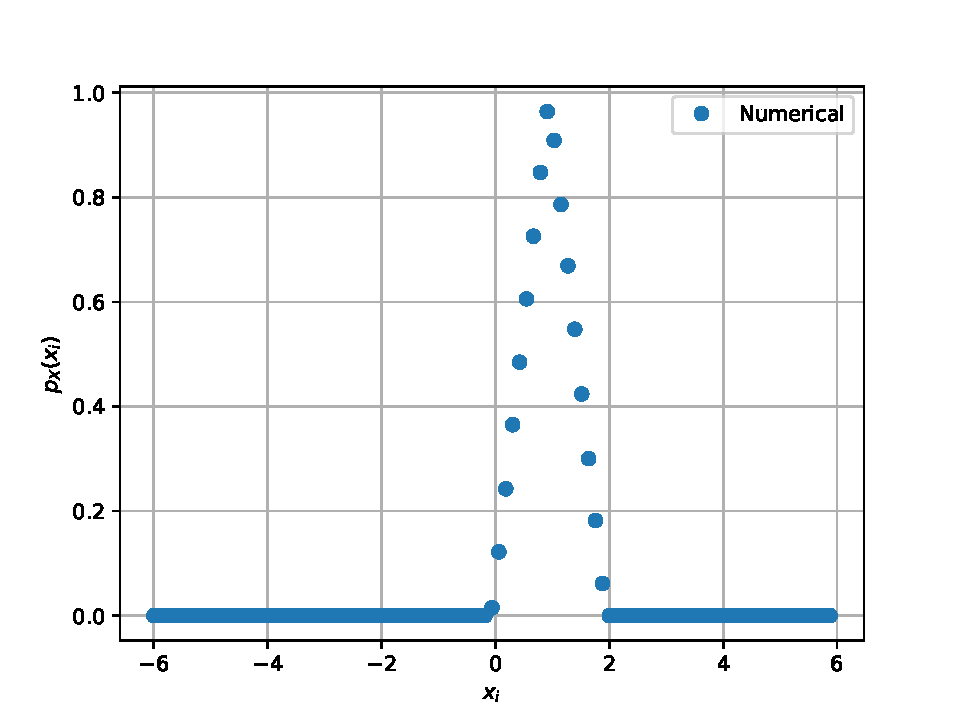
\includegraphics[width=\columnwidth]{../Figures/4_3_pdf}
\caption{PDF of T}
\label{fig:gauss_pdf}
\end{figure}

%4.4
\item Find the theoretical expressions for the PDF and CDF of T.\\
\solution 
\begin{align}
T &= U_1 + U_2 \\
p_T(t) &= p_{U_1} * p_{U_2} \\
p_T(t) &= \int_{-\infty}^{\infty} p_{U_1}(\tau)p_{U_2}(t - \tau) d \tau\\
p_T(t) &= 
\begin{cases}
0 & t \le 0\\
\vspace*{0.1in}
\int_{0}^{t} d \tau & 0 \le t < 1\\
\vspace*{0.1in}
\int_{t-1}^{1} d \tau & 1 \le t < 2\\
\vspace*{0.1in}
0 & t > 2
\end{cases}
\end{align}
For CDF :
\begin{equation}
F_T(x) = \int_{-\infty}^{x} p_T(t) dt
\end{equation}
From equation (4.5):
\begin{equation}
F_T(t) = 
\begin{cases}
0 & t \in (-\infty,0)\\
\frac{x^{2}}{2} & t \in (0,1)\\
\frac{-t^{2}}{2} + 2t -1 & t \in (1,2)\\
1 & t \in (2,\infty)
\end{cases} 
\end{equation}

%4.5
\item Verify results through plot\\
\solution\\ Link to the code for CDF:\href{https://github.com/anikettsatpute/Probability-and-Random-Variable-Assignment/blob/main/code/code4_5.py}{Pyhton code}\\
 Link to the code for PDF:\href{https://github.com/anikettsatpute/Probability-and-Random-Variable-Assignment/blob/main/code/code4_5_2.py}{Pyhton code}\\
\begin{figure}[h]
\centering
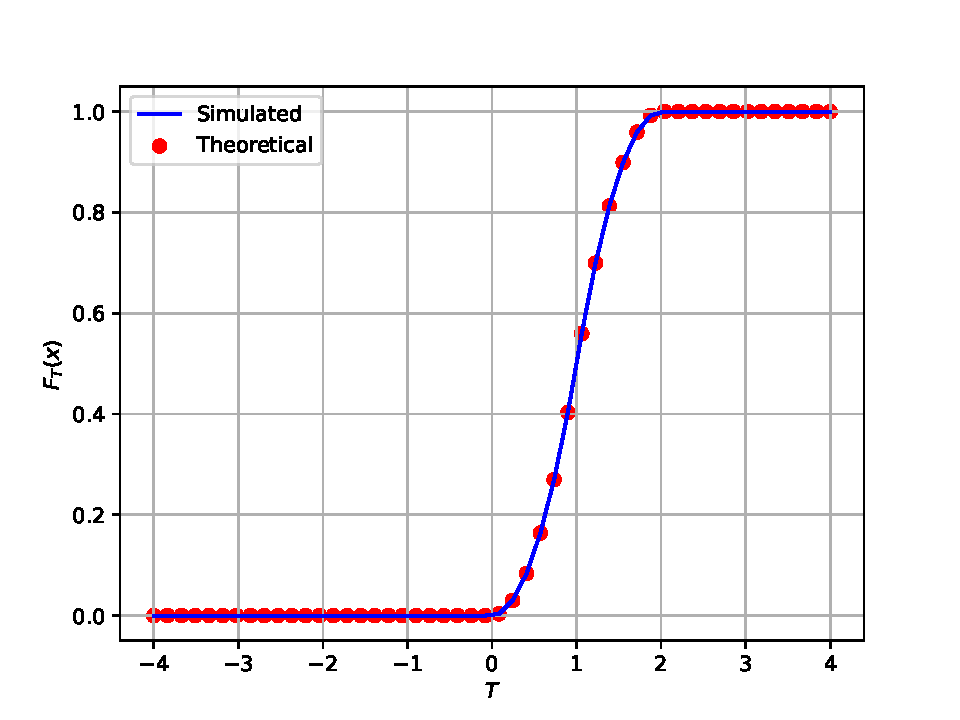
\includegraphics[width=\columnwidth]{../Figures/4_5_cdf}
\caption{Verification of CDF}
\label{fig:}
\end{figure}
\begin{figure}[h]
\centering
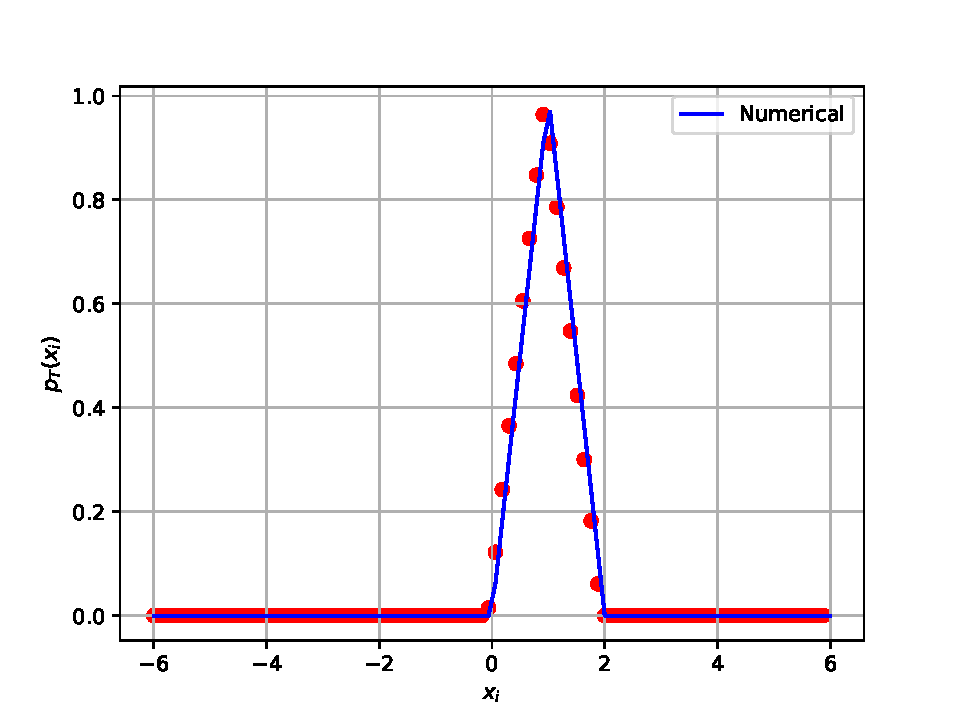
\includegraphics[width=\columnwidth]{../Figures/4_5_pdf}
\caption{verification of PDF}
\label{fig:}
\end{figure}
\end{enumerate}
\newpage
\section{Maximum Likelihood}
\begin{enumerate}[label=\thesection.\arabic*
,ref=\thesection.\theenumi]

%5.1
\item Generate equiprobable $X \in \{1 , -1\}$\\
\solution Link to the code :\href{https://github.com/anikettsatpute/Probability-and-Random-Variable-Assignment/blob/main/code/code5_1.c}{C code}\\
\vspace{0.2in}

%5.2
\item Generate
\begin{equation}
Y = AX + N,
\end{equation}
where A = 5 dB, and $N \sim \mathcal{N}(0,\,1)$.\\
\solution Link to the code :\href{https://github.com/anikettsatpute/Probability-and-Random-Variable-Assignment/blob/main/code/code5_2.c}{C code}\\
\vspace{0.2in}

%5.3
\item Plot Y using a scatter plot.\\
\solution Link to the code :\href{https://github.com/anikettsatpute/Probability-and-Random-Variable-Assignment/blob/main/code/code5_3.py}{Python code}\\

\begin{figure}[h]
\centering
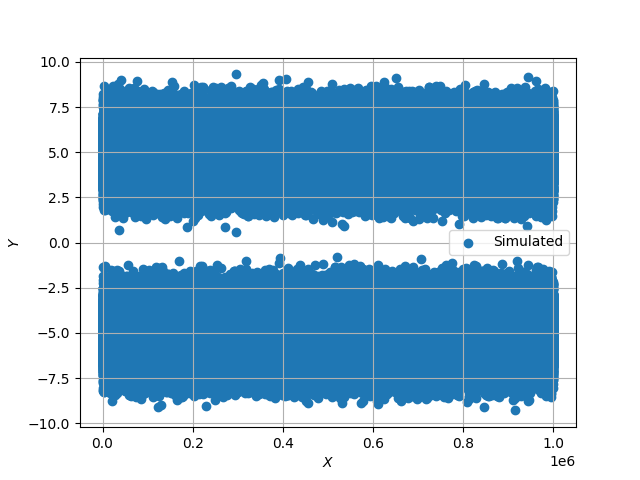
\includegraphics[width=\columnwidth]{../Figures/5_3_YvsX.png}
\caption{}
\label{fig:Y vs X}
\end{figure}

%5.4
\item Guess how to estimate X from Y.\\
\solution From Data and Plot generally:\\
\begin{equation} \label{eq:54}
X = 
\begin{cases}
1 & Y>0\\
-1 & Y<0
\end{cases}
\end{equation}

%5.5
\item Find
\begin{equation}
P_{e|0} = \Pr(\hat{X} = -1|X = 1)
\end{equation}
and
\begin{equation}
P_{e|1} = \Pr(\hat{X} = 1|X = -1)
\end{equation}
\solution Link to the code :\href{https://github.com/anikettsatpute/Probability-and-Random-Variable-Assignment/blob/main/code/code5_5.c}{C code}\\

\begin{figure}[h]
\centering
\includegraphics[width=\columnwidth]{../fig/screen55.png}
\caption{}
\label{fig:gauss_pdf}
\end{figure}
From the Figure above :
\begin{align*}
P_{e|0} = \Pr(\hat{X} = -1|X = 1) &= 0\\
P_{e|1} = \Pr(\hat{X} = 1|X = -1) &= 0
\end{align*}

%5.6
\item Find $P_e$ assuming that X has equiprobable symbols.\\
\solution Here.
\begin{equation}
\Pr(X=1) = \Pr(X=-1)=\frac{1}{2}
\end{equation}
Hence,
\begin{align*}
P_e &= \Pr(X=1) P_{e|1} + \Pr(X=-1) P_{e|0}\\
&=\frac{1}{2}(P_{e|1} + P_{e|0})\\
&= 0
\end{align*}

%5.7
\item Verify by plotting the theoretical $P_e$ with respect to A from 0 10dB.\\
\solution Link to the code :\href{https://github.com/anikettsatpute/Probability-and-Random-Variable-Assignment/blob/main/code/code5_7.py}{Python code}\\

\begin{figure}[h]
\centering
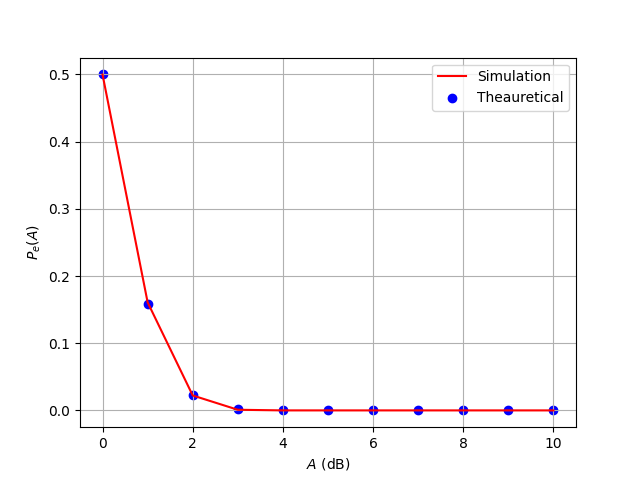
\includegraphics[width=\columnwidth]{../Figures/5_7.png}
\caption{}
\label{fig:gauss_pdf}
\end{figure}

%5.8
\item Now consider a threshold $\delta$ while estimating X from Y. Find the value of $\delta$ that maximizes the theoretical $P_e$\\
\solution From equation \eqref{eq:54}
Hence,
\begin{align*}
P_{e|0} &= \pr{\hat{X} = -1 | X = 1} \\
&= \pr{AX+N < \delta | X = 1} \\
&= \pr{N < \delta - A} \\
%&= \int _{-\infty} ^{\delta - A} \frac{1}{\sqrt{2\pi}} e^{-\frac{x^2}{2}} dx \\
%&= \int _{A - \delta} ^{\infty} \frac{1}{\sqrt{2\pi}} e^{-\frac{x^2}{2}} dx \\
&= Q_N(A - \delta) \\
\end{align*}
Where $Q_N$ is the $Q$-function of the normal distribution. Similarly,
\begin{align}
P_{e|1} &= Q_N(A+\delta) \\
\intertext{Therefore,}
P_e &= P_{e|0} \pr{X = 1} + P_{e|1} \pr{X = -1} \\ \label{eq:58}
&= \frac{1}{2}(Q_N(A - \delta) + Q_N(A + \delta)) \\
\end{align}
To find minima by differentiate wrt $\delta$
\begin{align*}
\frac{d(P_e)}{d \delta} &= \frac{1}{2}\frac{d}{d \delta}(Q_N(A - \delta)+Q_N(A+\delta))\\ 
&= \frac{1}{2\sqrt{2 \pi}}(e^-{\frac{(\delta - A)^2}{2}} - e^-{\frac{(\delta + A)^2}{2}}) = 0
\end{align*}
From above equation 
\begin{align*}
(\delta - A)^2 &= (\delta + A)^2\\
\intertext{Hence,}
\delta &= 0
\end{align*}

%5.9
\item Repeat the above exercise when
\begin{equation}
p_X(0) = p
\end{equation}
\solution From equation \ref{eq:58}
\begin{align*}
P_e &= P_{e|0}p + P_{e|1}(1-p)\\
&= Q_N(A-\delta) p + Q_N(A+\delta) (1-p)
\end{align*}
Again by differentiating,
\begin{equation*}
p\frac{1}{\sqrt{2 \pi}}e^-{\frac{(\delta - A)^2}{2}} - (1-p)\frac{1}{\sqrt{2 \pi}}e^-{\frac{(\delta + A)^2}{2}} = 0
\end{equation*}
By taking log,
\begin{align*}
\ln p- \frac{(\delta - A)^2}{2} &= \ln(1-p) + \frac{(\delta + A)^2}{2}\\
\delta &= \frac{1}{2A} \ln \frac{1-p}{p}
\end{align*}

%5.10
\item Repeat the above exercise using the MAP criterion.\\
% \solution Using Bayes' Theorem, we get
% \begin{align}
% 	&\pr{X = 1 | Y = y} \nonumber \\
% 	&= \frac{\pr{N = y - A | X = 1}\pr{X = 1}}{\pr{Y = y}} \\ 
% 	&= \frac{pf_N\brak{y - A}}{pf_N\brak{y - A} + \brak{1 - p}f_N\brak{y + A}} \\
% 	&= \frac{p}{p + \brak{1 - p}e^{-2yA}} 
% \end{align}
% and
% \begin{align}
% 	&\pr{X = -1 | Y = y} \nonumber \\
% 	&= \frac{\pr{N = y + A | X = -1}\pr{X = -1}}{\pr{Y = y}} \\ 
% 	&= \frac{\brak{1 - p}f_N\brak{y + A}}{pf_N\brak{y - A} + \brak{1 - p}f_N\brak{y + A}} \\
% 	&= \frac{1 - p}{\brak{1 - p} + pe^{2yA}} 
% \end{align}
% Hence, 
% \begin{align}
% 	\frac{p}{p + \brak{1 - p}e^{-2yA}} &\gtrless \frac{1 - p}{\brak{1 - p} + pe^{2yA}} \\
% 	\implies p^2e^{2yA} &\gtrless \brak{1 - p}^2e^{-2yA} \\
% 	\implies y &\gtrless \frac{1}{2A}\ln{\brak{\frac{1 - p}{p}}}
% \end{align}

\end{enumerate}

\end{document}
